\chapter{Improvement of Visual Odometry}\label{Chap:Imp}
Above the procedure of self-localization was described in general. Particle filter require sensor measurement to calculate the weighting for each particle and Unscented Kalman filter demands the sensor measurements to update the motion predictions. Visual odometry is a widely used with strong functions sensor measurement method, which is applied in this situation and provides the measurement for each kind of filter. So the accuracy of pose estimated by visual part will definitely have an obvious influence on the final result. This chapter will introduce what knowledge of the sensor measurement can provide and how the sensor measurement take place. 
\section{The current method}
\subsection{Visual odometry procedure}
There are several sensors to acquire information from the environment on NAO: camera, microphone and sonar. From them only the camera is adopted, since the environment of the soccer match will be quite complicated, for example:
\begin{itemize}
    \item The white border lines and green field are on the same plane.
    \item The goal posts are perhaps too far away from the robots sometimes.
    \item There are 6 moving robots on the field, which the opponents are distinguished from our teammates only by colors.
    \item The ball is small and the detection of a ball requires high precision.
\end{itemize}
So based on above reasons, the another sensors are not qualified for the requirements. However, the camera is suitable for each specific task and the computer vision skill as well as visual odometry are being perfect so far.

There two cameras on the NAO's head which can provide large FOV. Several tasks such as image preprocessing, feature detection(including: line perception, penalty mark perception, ball perception) and data association will be performed on the image gathered by each camera. B-Human's current vision system provides a variety of perceptions that have all been integrated into the sensor model: goal posts (ambiguous as well as unambiguous ones), line segments (of which only the endpoints are matched to the field model), line crossings (of three different types: L, T, and X ), and the center circle \cite{BHumanCodeRelease2012}. These features can be associated to the feature detected in pixel images. The detailed of these tasks will not be mentioned in my part of report, which are introduced by my teammates. My work is that suppose the the feature detection and data association have been finished.

Based on feature detection and data association, the corresponding point pairs have been already found. For example the goal post in figure i. whose coordinate in the homogeneous global 3D world could be represented as $(X,Y,0,1)^T$. And the corresponding homogeneous coordinate in pixel coordinate can be written as $(x,y,1)^T$. Since the camera calibration matrix, including both intrinsic and extrinsic calibration parameters, has been acquired through camera calibration before each match. Assuming the camera model as pinhole camera model shown in \fref{fig: camera} \cite{hartley2003multiple}: 
\[ % without number
\mathbf{x} = \mathbf{K} \cdot \mathbf{X}_{cam}
\]
\begin{figure}[!htb]
    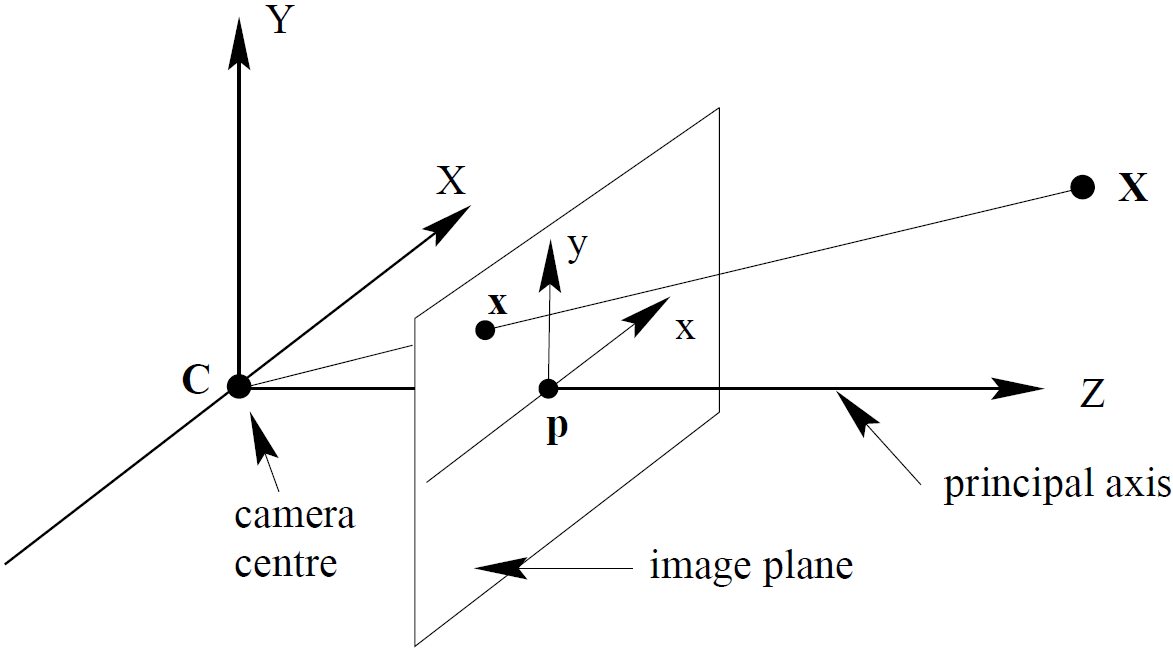
\includegraphics[width=0.4\textwidth]{pics/cameramodel.png}
    \centering
    \caption{Pinhole camera model}
    \label{fig: camera}
\end{figure}

So we could get the corresponding 3D goal post coordinate in the ideal camera frame. Since we know the geometrical value of NAO's body construction, we can transform the coordinates into the robot frame, which is shown in the \fref{fig: trans.sub.1}
\begin{figure}[tbp]
\centering
\subfigure[Coordinate transform]{
\label{trans.sub.1}
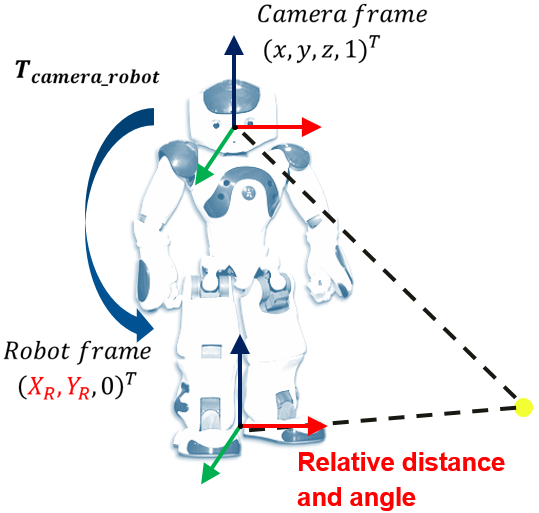
\includegraphics[width=0.45\textwidth]{pics/coordinate_transform.png}}
\subfigure[Relative pose to landmark]{
\label{trans.sub.2}
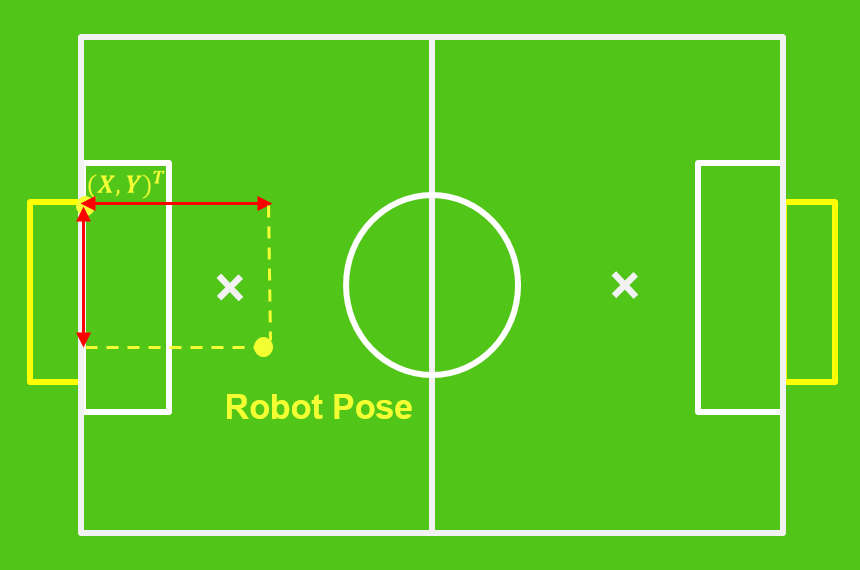
\includegraphics[width=0.45\textwidth]{pics/relative.png}}
\caption{Pose estimation}
\label{fig: trans}
\end{figure}
Based on this, we could get the related distance between robot and the goal post in robot frame. At the same time, the precise location of goal post in the global field is also known. So we could calculate the robot pose from this above information.
\subsection{Current problem}
In the process of transforming the coordinate from camera frame into robot frame, the current method only use a constant transform. However when robot is walking, it cannot always be extremely vertical to the ground. The central line of its body and camera on the head will have an arbitrary angle of tilt. Also due to detecting of the environment, robot always turn around its head or even look up and down, but this information will also create bias by coordinate transforming. Then it will cause a bias on the camera frame transform, which is shown in \fref{fig: error}. This error between the real robot base coordinate and the result calculated by the constant transform will further affect the pose estimation. 
\begin{figure}[!htb]
    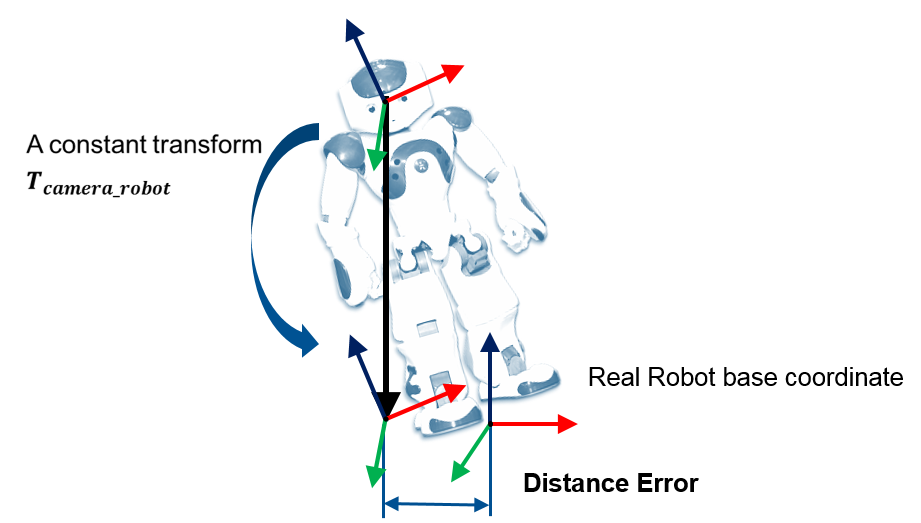
\includegraphics[width=0.7\textwidth]{pics/error.png}
    \centering
    \caption{Position error by a constant transform}
    \label{fig: error}
\end{figure}\\

\section{PnP Pose estimation}
Since the current method contains the tilting and shaking error so I apply the PnP method \cite{ETHPnP} which could eliminate the error by consider the transform in a more direct way. Reconsidering corresponding point pair $\mathbf{x}:=(x,y,1)^T$ in pixel coordinate and $\mathbf{X}:=(X,Y,0,1)^T$ in 3D global space. They should have this following relationship \eqref{relation}:
\begin{equation}
\mathbf{x} = \mathbf{T}_{image2field} \cdot \mathbf{X}_{field} \label{relation}
\end{equation}
And the transform matrix $\mathbf{T}_{image2field}$ could be represented as three parts: 
\begin{equation}
\mathbf{T}_{image2field}=\mathbf{K} \cdot \mathbf{T}_{camera2robot} \cdot \mathbf{T}_{robot2field} \label{transform}
\end{equation}
In \eqref{transform} what we can figure out from the corresponding point pairs is $\mathbf{T}_{image2field}$, and what we want to know is $\mathbf{T}_{robot2field}$. If we know the $\mathbf{T}_{robot2field}$ then we could directly read robot pose from this matrix. Also, the camera calibration matrix $\mathbf{K}$ is also already known because the calibration has been done before each match. 
$\mathbf{T}_{robot2field}$ can also be represented as \eqref{Trf}:
\begin{equation}\mathbf{T}_{robot2field}=
\begin{bmatrix}
\mathbf{R} & \mathbf{T}
\end{bmatrix}=
\begin{bmatrix}
cos\alpha & sin\alpha & 0 & T_x\\
-sin\alpha & cos\alpha & 0 & T_y\\
0 & 0 & 1 & 0
\end{bmatrix} \label{Trf}
\end{equation}

There are 4 unknown parameters in \eqref{Trf}, so at least 2 pairs of corresponding points are required to solve the equation. The 2 pairs of corresponding points can be selected by two goal posts or the start and end point of a specific line. Suppose $\mathbf{M}:=\mathbf{K} \cdot \mathbf{T}_{camera2robot}$, elements in $\mathbf{M}$ are all known values, so the equation can be written as \eqref{Trf2}:
\begin{equation}\mathbf{x}=\mathbf{M} \cdot
\begin{bmatrix}
\mathbf{R} & \mathbf{T}
\end{bmatrix} \cdot \mathbf{X} =\mathbf{A}\cdot \mathbf{X}
\label{Trf2}
\end{equation}

\begin{equation}[\mathbf{x_1} \quad \mathbf{x_2}]=
\mathbf{A}\cdot [\mathbf{X_2} \quad \mathbf{X_2}]
\label{Trf3}
\end{equation}

So, in \eqref{Trf3} it shows the how does two pairs of corresponding points calculate matrix $\mathbf{A}$ which contains four unknown parameters. If we have more than 4 pairs of corresponding points, SVD method for minimum solution finding could be applied.





